%\documentclass[11pt, oneside]{article}   	
%\usepackage{geometry}    
%\geometry{letterpaper}                 		
\input preamble.tex
\newcommand{\ig}[2][width=4in]{\includegraphics[#1]{#2}}    		
\usepackage{graphicx}					
\usepackage{amssymb}
\usepackage{pgfplotstable}
\usepackage{float}
\usepackage{caption}
\captionsetup[table]{justification=justified,singlelinecheck=false, position=bottom}
\begin{document}

\header {\today}							
\title{Muon Lifetime}
\author{Ekta Patel \& Brandon Booth-Dunbar}

\section{Abstract}
%Ekta
\begin{em} Positively charged muons reach the Earth via cosmic ray showers.When they decay, the muons break down into a positron, an electron neutrino and a muon neutrino.The goal of the experiment is to measure the lifetime of the muon by detecting and stopping a positive muon in an aluminum slab and then consequently detected the positron that it leaves behind when it decays.The distribution of the difference in detection times can be used to determine the muon lifetime.
\end{em}

\section{Theory}
%Brandon

\section{Experimental Methods}
%Ekta, but I (Brandon)  will make the figures
\subsection{Apparatus}
\indent  \indent As a positively charged muon reaches the Earth and hits the scintillation detector, a small flash of light is observed due to the plastic sheet of the scintillator. The photomultiplier then changes the flash of light into a pulse of electrons which then travels to an amplifier/discriminator that filters away the noise from the detector in addition to strengthening the incoming pulse of electrons. The amplifier/discriminator then feeds the output pulse into the coincidence circuit to ensure that only the positrons and muon electrons are detected. 
\newline \indent We want to start a clock when a positive muon is detected in the aluminum slab and stop the clock when the positron is detected from the muon decay. The distribution of a very large number of delay times, created by the `start' and `stop' of the detections, will be used to determine the lifetime of the muon. 
\newline \indent In our setup, we have three photomultipliers($A, B, C$), two of which will trap the muon long enough for it to decay and a third that will help in the detection of the positron. We use the $A$ and $B$ photomultipliers to detect and trap the muon. When $A$ and $B$ are triggered, but not C, the clock will start to count until either $B$ or $C$ is triggered again by the positron and stops the clock. We do not want all three photomultipliers to be triggered when the muon is detected because the time delay will be irrelevant since the clock will start and stop almost instantaneously. We need the muon to be trapped by two photomultipliers and the resulting positron to be detected by one of the photomultipliers. Therefore, the start and stops of the clock correspond to:
\begin{equation} start: \textbf A\;and\; \textbf B \end{equation}
\begin{equation} stop: \textbf B\; or\; \textbf C \end{equation}
Though we choose to setup our apparatus in this way, there is also another possibility in which the $A$ and $B$ photomultipliers are used to detect the muon but then only $B$ exclusively or C detect the positron ($B$ XOR $C$). This setup guarantees that the clock would only be stopped if either $B$ or $C$ were activated, but not both since the positron only travels either up or down through the apparatus as the muon decays. However, we do not choose to set up our experiment that way because it is not likely that another muon will be detected faster than in the time scales that we are observing. Since the muon realistically only takes about 2 $\mu$s to decay, a false trigger of photomultiplier $B$ would have to take place in that much time or less. During calibration, we find that $B$ receives about 50 counts per second. Therefore, it is triggered about 10$^{-4}$ times within the muon lifetime of approximately 2$\mu$s, making it nearly impossible to detect a muon in the same time span that one is already decaying. It is also important to remember that muons are only reaching the Earth's surface at a  muon sea level flux of only 1 /cm$^2$/minute or about one muon every 6x10$^7\mu$s.
\newline \indent As the photomultipliers are triggered, Time-to-Amplitude Converter converts the times between each `start' and `stop'  to voltages. These voltages are then recorded by the Multi-Channel Analyzer which uses the computer to bin the data into a histogram based on the strengths of voltages which correspond to the lengths of times taken for each detected muon to decay. It is important to remember that the muon flux at sea level is only 1 /cm$^2$/minute, so we will need to take data sets that stretch over several days to a few weeks to get a good distribution of delay times. A good representation of the apparatus from the photomultiplier tubes to the logic setup and ending with the final output of time delays is shown in the figure below: 


\begin{figure}[H]
\begin{center}
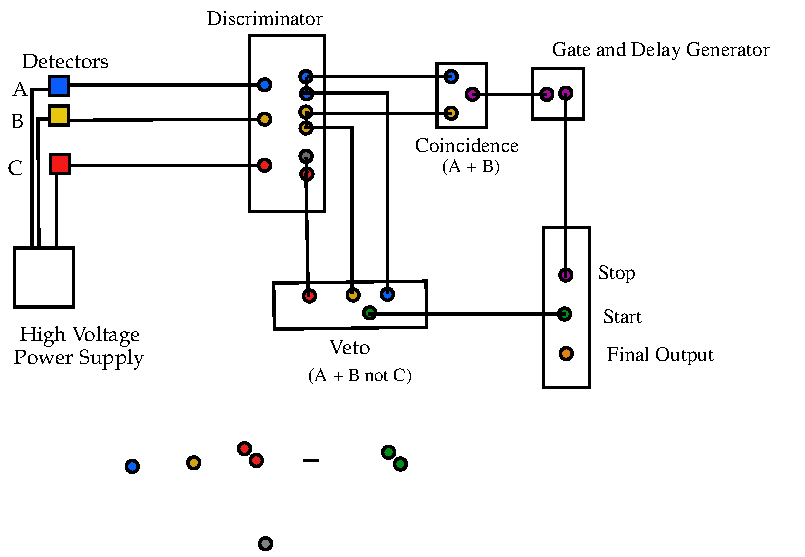
\includegraphics[width=6 in]{ML-figure1.pdf}
\caption{The apparatus}
\end{center}
\end{figure}

\subsection{Procedure}
\indent \indent To obtain the clearest and best signals possible for muon detection, we must first plateau each photomultiplier so that the signal to noise ratio of each one is as ideal as possible. The noise level will increase exponentially with time, whereas the signal will reach a maximum value and then plateau. This plateau region is the voltage that we want to achieve for photomultipliers A, B and C. We use an electron source of Bismuth to plateau the detectors by placing the source in approximately the same place on the aluminum slab leading to the photomultipliers while plugging in each one individually to the counter to see the counts detected just from the source's presence over one second time intervals. We started at a voltage of about 1000V for each of the photomultipliers and increased by 100V until we reached 1400V. At that point, we increased in increments of 10V as to not exceed the maximum voltage of 1500V. The table below gives the results of the voltages at which we found the plateaus in counts and the corresponding counts both with and without a source present. 
\begin{table}[h]
\begin{center}
\begin{tabular}{|c|c|c|c|} \hline
Photomultiplier & Voltage & Counts w/ Source & Counts w/o Source \\ \hline
A & 1450 V & 295 & 50 \\ \hline
B & 1450 V & 440 & 140 \\ \hline
C & 1470 V & 420 & 80\\ \hline

\end{tabular}
\caption{Values chosen for power supplied in voltage to each photomultiplier, including the number of counts with a Bismuth source on the apparatus to no source on the apparatus. The time interval for the number of counts for all three photomultipliers is 1 second.}
\end{center}
\end{table}

Data sets are taken on time scales of several days to a few weeks to obtain a result with reasonable precision. As discussed earlier, muons are not reaching the Earth at a very high rate, but furthermore, they are not being stopped in our apparatus 100\% of the time that they reach the ground. Therefore, longer time scales are more suitable to analyze the range of time delays that are used to determine the muon lifetime. After data has been obtained, it is important to calibrate the Time-Amplitude Converter to remove extraneous results that may be time delays that are too large to be feasible with the rest of the data set or even too small. The following table shows corresponding values for the amount of time lapsed in comparison to the matching bin number. The total number of bins observed with both the one week long and two week long data set is set to be 2048. Therefore, about 10\% of the total number of bins represent time delays of 1$\mu$s or less, whereas about 60\% of the bins correspond to time delays of 4$\mu$s or greater. 
\begin{table}[h]
\begin{center}
\begin{tabular}{|c|c|}\hline
Time & Bins\\ \hline
1 $\mu$s & 204.85\\ \hline
2 $\mu$s & 402 \\ \hline
3 $\mu$s & 608 \\ \hline
4 $\mu$s & 809 \\ \hline
\end{tabular}
\caption{Number of microseconds for which the calibration of the data has been determined to be binned. The number of bins given represents the number of bins from the zeroeth bin in our data run. The total number of bins  is 2048.}
\end{center}
\end{table}

% 2- 402 bins
% 3 -- 608
%4-- 809 bins over


\section{Results \& Discussion}
%Brandon

\section{Conclusion}
%Ekta
% final time
%how errors could be minimized or eliminated.

\begin{thebibliography}{99}
\bibitem{electron}Sleator, Tycho, and Budick, Burton, \begin{em}Muon Lifetime. \end{em}Experimental Physics. V85.0112. Spring, 2012.
\end{thebibliography}

\newpage \LARGE{Appendix}

\end{document}  
